\section{Solving Identification with a Control Function}
\label{sec:controlfun}
If your goal is to estimate CM effects, and you could control for unobserved selection into $D_i$, then you would.
This ideal example would yield unbiased estimates
% Alas, $U_i$ is by definition unobserved.
The control function method takes this insight seriously, providing conditions to model the implied unobserved confounder, $U_i$, and then control for it.\footnote{
    This section does not improve on the control function approach, instead only noting its utility to solve the identification problem of CM in a natural experiment setting.
}

Suppose the vector of control variables $\vec X_i$ has at least two entries;
denote $\vec X_i^{\text{IV}}$ as one entry in the vector, and $\vec X_i^-$ as the remaining rows.

\begin{definition}
    \label{dfn:controlfun-assumptions}
    Control function assumptions.
    \begin{align}
        \label{eqn:firststage-monotonicity}
        &\Probgiven{ D_i(1) \geq D_i(0) }{\vec X_i} = 1    \\
        \label{eqn:controlfun-iv}
        &\vec X_i^{\text{IV}} \text{ has the property }
        \partialdiff[\mu(\vec X_i)]{\vec X_i^{\text{IV}}} = 0 < \partialdiff[D_i(z')]{\vec X_i^{\text{IV}}}, \textnormal{ for } z' = 0, 1.
    \end{align}
\end{definition}
Assumption \ref{dfn:controlfun-assumptions}\eqref{eqn:firststage-monotonicity} is the (conditional) monotonicity assumption \citep{imbens1994identification}, which is untestable but acceptable in many empirical applications.
Assumption \ref{dfn:controlfun-assumptions}\eqref{eqn:controlfun-iv} is assuming that an instrument exists, which satisfies an exclusion restriction (i.e., not impacting mediator gains $\mu$), and has a non-zero influence on the mediator (i.e., strong first-stage).
The exclusion restriction is untestable, and must be guided by domain-specific knowledge; strength of the first-stage is testable, and must be justified with data by methods common in the IV literature.

Write $K_i$ for the error in predicting the mediator with observed data, as a function of the instrument $\vec X_i^{\text{IV}}$ and remaining controls $\vec X_i^-$.
$K_i$ serves as the control function in this setting.
\[ K_i = D_i - \Egiven{D_i}{Z_i, \vec X_i^{\text{IV}}, \vec X_i^-} \]

\begin{theorem}
    \label{thm:controlfun}
    If \ref{dfn:controlfun-assumptions}\eqref{eqn:firststage-monotonicity} and \ref{dfn:controlfun-assumptions}\eqref{eqn:controlfun-iv} hold, then the average potential outcomes (and thus, the ADE and AIE) are identified by a control function approach.
    \[ \Egiven{Y_i}{Z_i = z', D_i = d', \vec X_i^-, K_i}
        = \Egiven{Y_i(z', d')}{\vec X_i^-, K_i}
        , \;\; \text{ for } z', d' = 0,1. \]
\end{theorem}
\begin{proof}
    Special case of \citet[Theorem~1]{imbens2009identification}; see \autoref{appendix:controlfun-proof}.
\end{proof}

Assumption \ref{dfn:controlfun-assumptions}\eqref{eqn:firststage-monotonicity} guarantees that mediator $D_i(.)$ can be represented by a selection model \citep{vytlacil2002independence}, and \ref{dfn:controlfun-assumptions}\eqref{eqn:controlfun-iv} pins down a control function to identify the selection model.

Two sentences here describing the identification results.
link to other references in 

Writing here about how the Roy model is solves with this, and the instrument impacts costs of mediator take-up.


\subsection{Estimation}




Write here about the two-stage estimation.
Indeed, CM requires two-stage estimation already, so the control function is a natural extension.

There are practical concerns for using the control function approach.
\begin{itemize}
    \item Estimate first-stage non-parametrically --- and thus needs a large large sample size (e.g., Biobank).  Although CM methods are already low in efficients
    \item Control function non-parametric in second-stage
    \item SEs with bootstrap (even worse with a burdensome non-parametric method in both stages)
\end{itemize}

\subsection{Simulation Evidence}
The following simulation gives an example to show how the control function works in practice.
Data observed to the researcher $Z_i, D_i, Y_i, \vec X_i$ are drawn from the following data generating processes, for $i = 1, \hdots, N$.
\begin{align*}
    Z_i \sim \text{Binom}\left(0.5 \right),
    \;\; \vec X_i^- \sim N(4, 1),
    \;\; \vec X_i^{\text{IV}} \sim \text{Binom}\left( 0.5 \right), \\
    \left[ U_{0,i}, U_{1,i} \right]' \sim
    \text{BivariateNormal}\left( 0, 0, \sigma_0, \sigma_1, \rho \right),
    \;\; U_{C,i} \sim N(0, 0.25).
\end{align*}
Additionally, suppose each $i$ chooses to take mediator $D_i$ based on the costs and benefits (i.e., a Roy model), with following definitions for each $z', d' = 0, 1$.
\begin{align*}
    \mu_{d'}\left(z' ; \vec X_i \right) = \vec X_i^- + \left( z' + d' + z' d' \right),
    \;\; \mu_{C}\left(z' ; \vec X_i \right) = 3z' + \vec X_i^- - \vec X_i^{\text{IV}}.
\end{align*}
Following \autoref{sec:selection}, these data have the following outcome equations:
\begin{align*}
    D_i &= \indicator{-3Z_i - \vec X_i^{\text{IV}} + \vec X_i^- \geq U_{0,i} - U_{1,i}},  \\
    Y_i &= Z_i + D_i + Z_i D_i + \vec X_i^-
        + \left( 1 - D_i \right) U_{0,i} + D_i U_{1,i}.
\end{align*}
In this setting the error terms $U_{i, 0}, U_{i, 1}$ determine the bias in OLS estimates of the ADE and AIE, so the bias varies for different values of the DGP parameters $\rho \in [-1, 1]$ and $\sigma_0, \sigma_1 \geq 0$.

% \textbf{To-do:} write the formula for main confounders, $\E{U_{0,i}}{D_i = 0}$ and $\E{U_{1,i}}{D_i = 1}$, which are the bias terms, and how they depend on $\rho, \sigma_0, \sigma_1$.

\begin{figure}[h!]
    \caption{OLS versus Control Function Estimates of CM Effects.}
    \begin{subfigure}[c]{0.475\textwidth}
        \centering
        \caption{ADE.}
        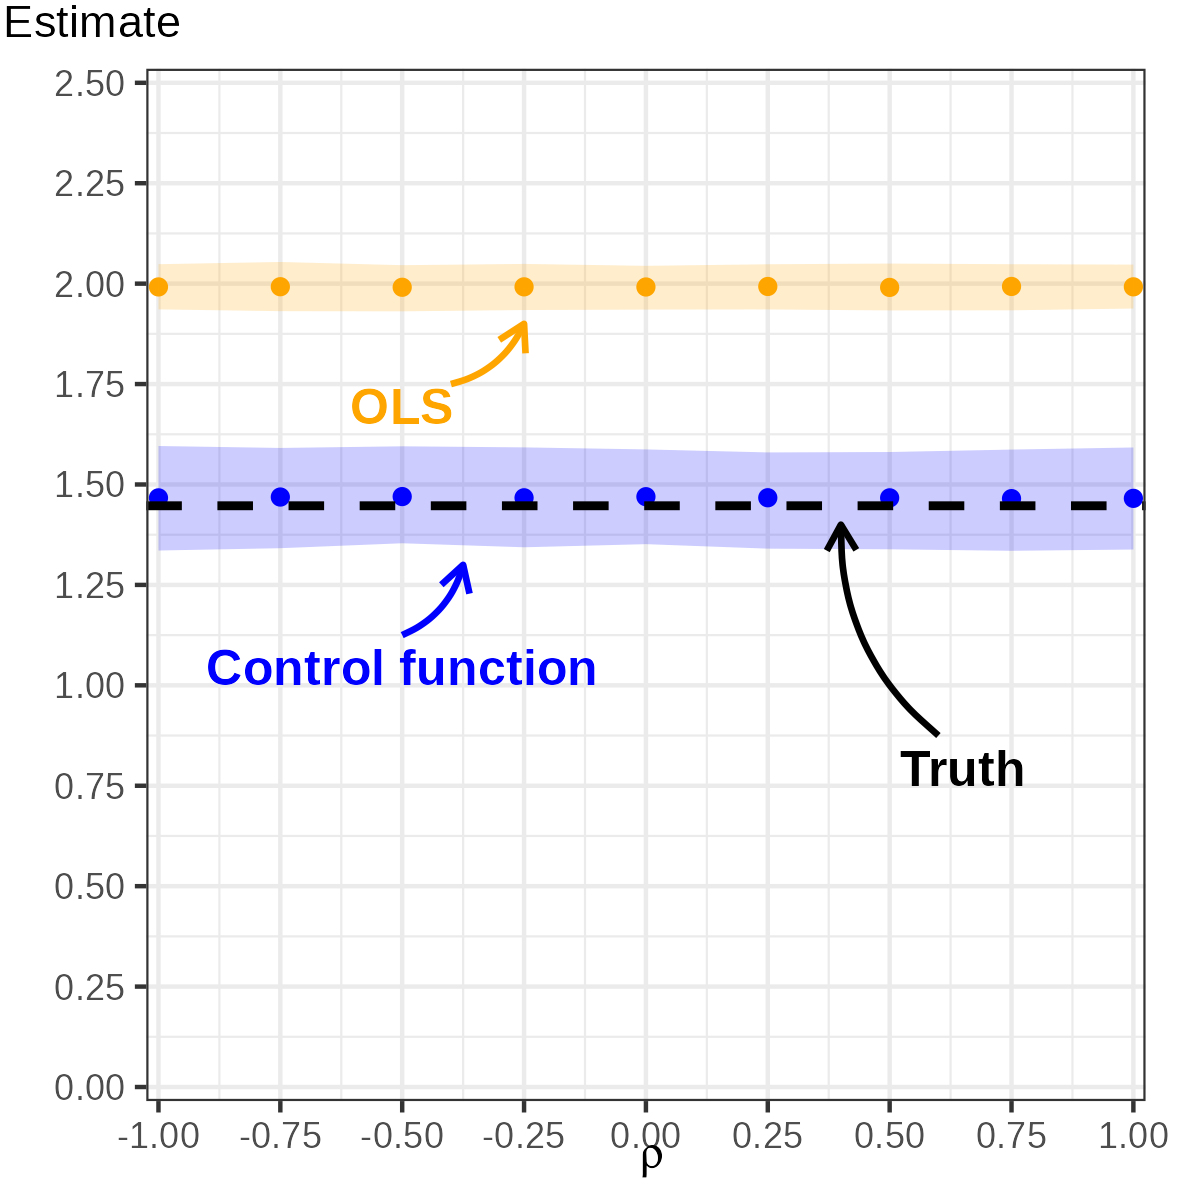
\includegraphics[width=\textwidth]{
            ../programs/simulations/sim-output/rho-directeffect-bias.png}
    \end{subfigure}
    \begin{subfigure}[c]{0.475\textwidth}
        \centering
        \caption{AIE.}
        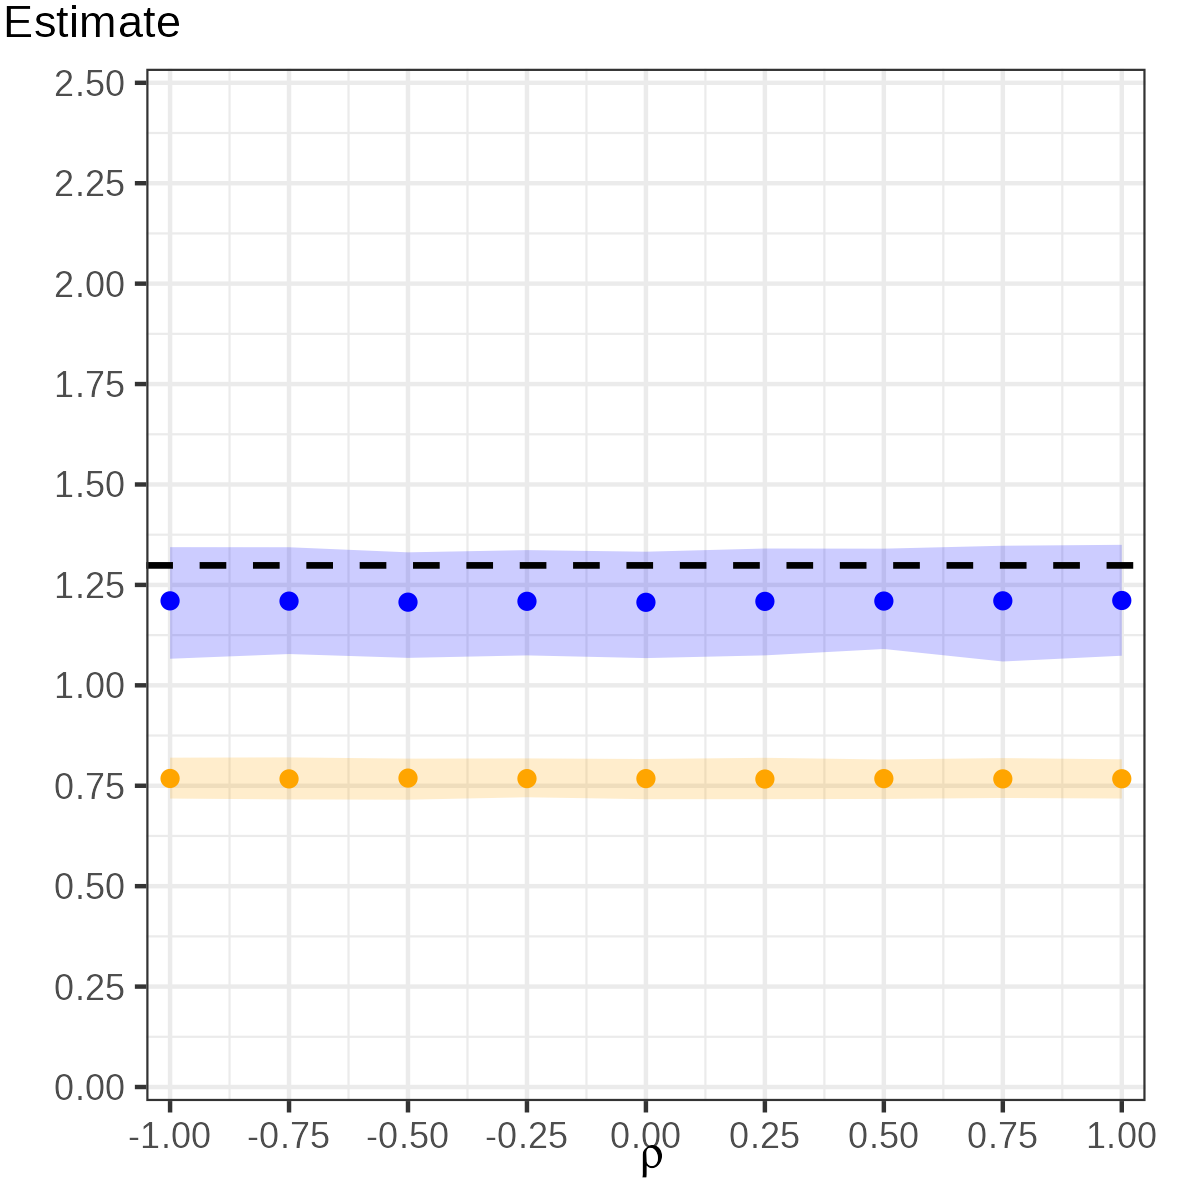
\includegraphics[width=\textwidth]{
            ../programs/simulations/sim-output/rho-indirecteffect-bias.png}
    \end{subfigure}
    \label{fig:rho-bias}
    \justify
    \footnotesize    
    \textbf{Note:}
    These figures show the OLS and control function estimates of the ADE and AIE, for $N = 10,000$ sample size.
    The black dashed line is the true value, points are points estimates from data simulated with a given $\rho$ value and $\sigma_0 = 1, \sigma_1 = 2$, and shaded regions are the 95\% confidence intervals.
    Orange are the OLS estimates, blue the control function approach described herein.
\end{figure}

